\documentclass{beamer}
\usepackage{graphicx}
\usepackage{amsmath, esint}

\usepackage{ragged2e}
\usepackage{tikz}
\usetikzlibrary{arrows,shapes}

\usepackage{listings}
\lstset{escapeinside={@(}{)@}}
\usepackage{algorithm}
\usepackage{algorithmic}

\usepackage{tabularx}
\newcolumntype{Y}{>{\centering\arraybackslash}X}

% \usepackage{minted}
\usepackage{xcolor} 
\definecolor{LightGray}{gray}{0.975}

\usepackage{amssymb}

\def\ojoin{\setbox0=\hbox{$\bowtie$}%
  \rule[-.02ex]{.25em}{.4pt}\llap{\rule[\ht0]{.25em}{.4pt}}}
\def\leftouterjoin{\mathbin{\ojoin\mkern-5.8mu\bowtie}}
\def\rightouterjoin{\mathbin{\bowtie\mkern-5.8mu\ojoin}}
\def\fullouterjoin{\mathbin{\ojoin\mkern-5.8mu\bowtie\mkern-5.8mu\ojoin}}

%\usetheme{Warsaw}
\usefonttheme{serif} 

\title[Chapter 7]{Database System Concepts, $7^{th}$ Edition \\ Chapter 7: Relational Database Design}
\author{Silberschatz, Korth and Sudarshan}
\date{\today}

\setbeamertemplate{navigation symbols}{}%remove navigation symbols

\defbeamertemplate*{footline}{shadow theme}
{%
  \leavevmode%
  \hbox{\begin{beamercolorbox}[wd=.5\paperwidth,ht=2.5ex,dp=1.125ex,leftskip=.3cm plus1fil,rightskip=.3cm]{author in head/foot}%
    \usebeamerfont{author in head/foot} Database System Concepts \hfill \insertshorttitle
  \end{beamercolorbox}%
  \begin{beamercolorbox}[wd=.5\paperwidth,ht=2.5ex,dp=1.125ex,leftskip=.3cm,rightskip=.3cm plus1fil]{title in head/foot}%
    \usebeamerfont{title in head/foot} \hfill \insertframenumber\,/\,\inserttotalframenumber%
  \end{beamercolorbox}}%
  \vskip0pt%
}

\AtBeginSection[]
{
     \begin{frame}<beamer>
     \frametitle{Plan}
     \tableofcontents[currentsection]
     \end{frame}
}

\newcommand{\toRight}[1]{
    \begin{FlushRight}
        {\tiny #1}
    \end{FlushRight}
} % Align to right

\begin{document}

\frame{\titlepage}

\begin{frame}{Database System Concepts}
    \centering
    
\includegraphics[width=0.5\textwidth]{figures/book_cover.jpg} \\
    \vspace{5mm}
    {
        \tiny
        Content has been extracted from \textit{Database System Concepts}, Seventh Edition, by Silberschatz, Korth and Sudarshan. Mc Graw Hill Education. 2019.\\
        Visit \url{https://db-book.com/}.\\
    }
\end{frame}

\section{Features of Good Relational Design}

\begin{frame}{Features of Good Relational Designs}
    \centering
    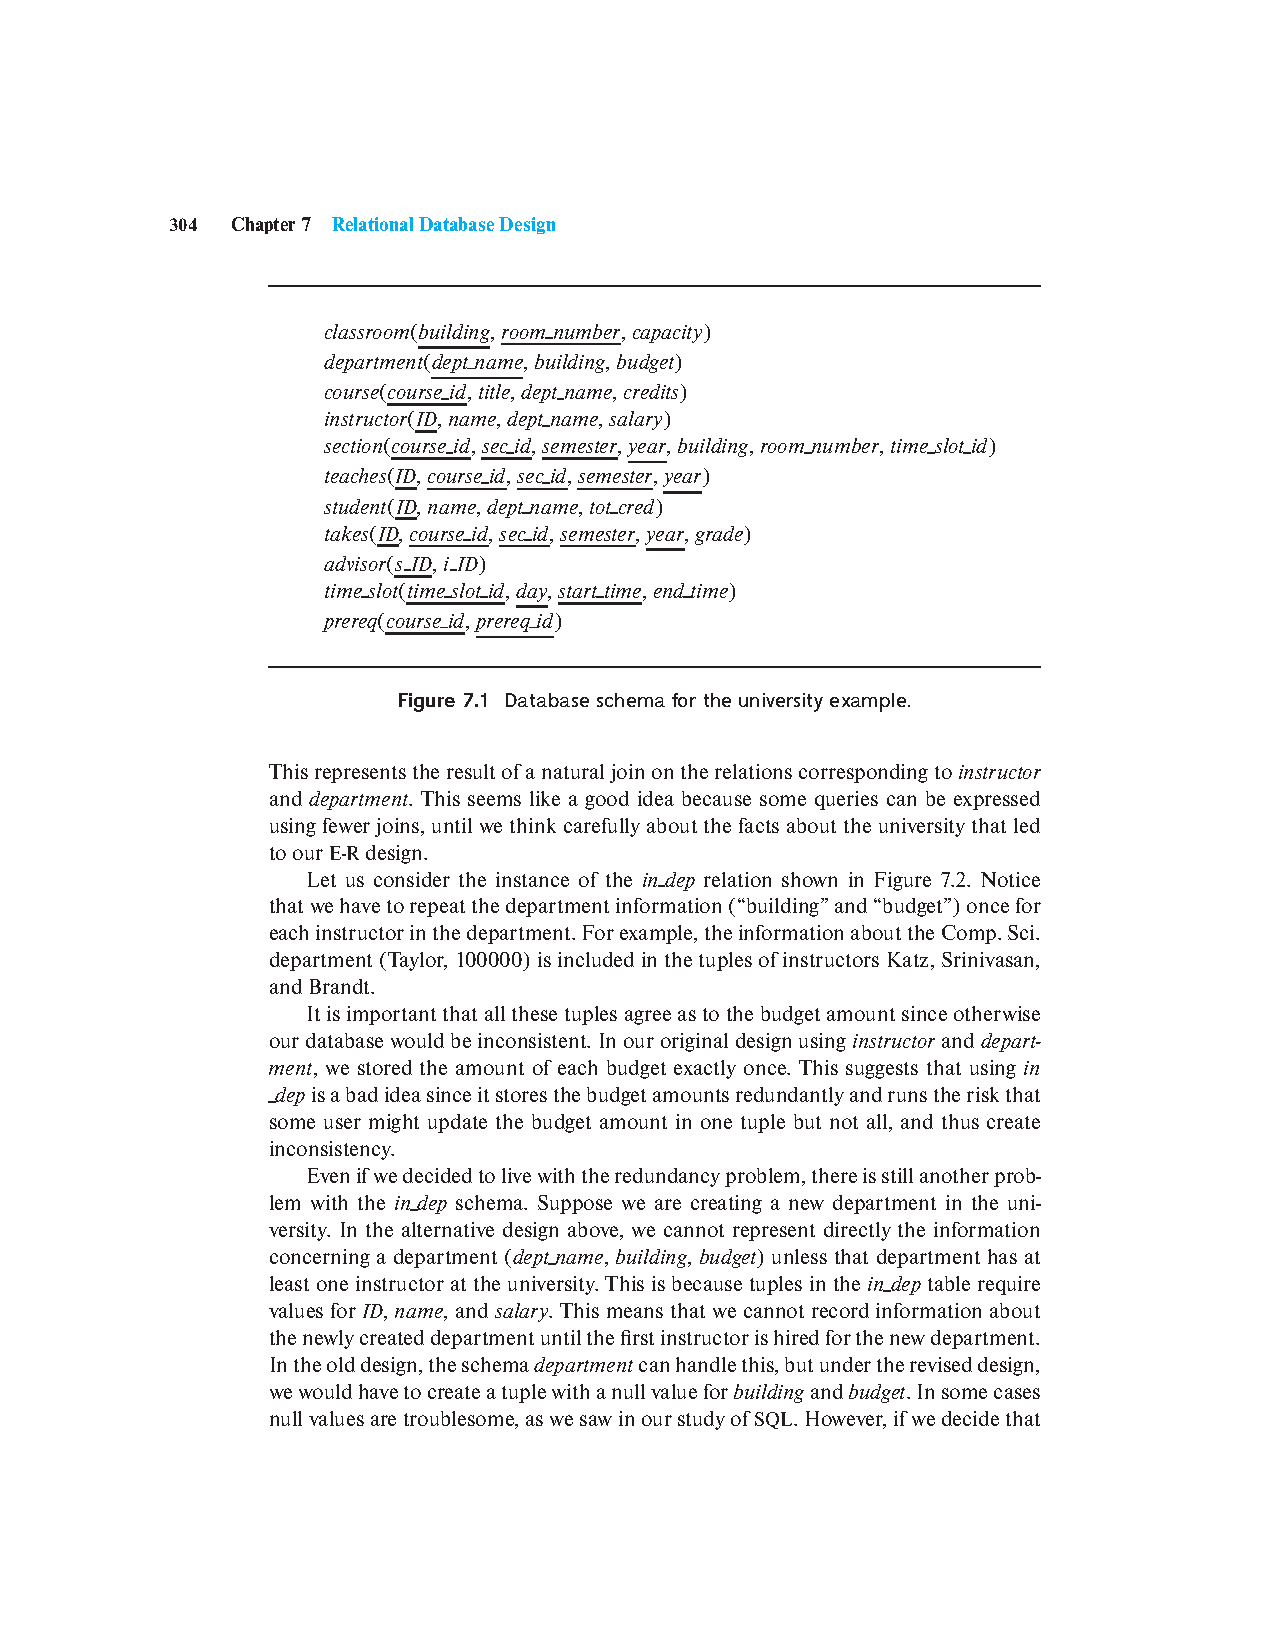
\includegraphics[width=\textwidth, trim={5cm 15.75cm 4cm 4.75cm}, clip]{figures/p304_schema}
\end{frame}

\begin{frame}{Features of Good Relational Designs}
    \begin{itemize}
        \item Suppose we combine \textit{instructor} and \textit{department} into \textit{in\_dep}, which represents the natural join on the relations \textit{instructor} and \textit{department}.
            \begin{center}
                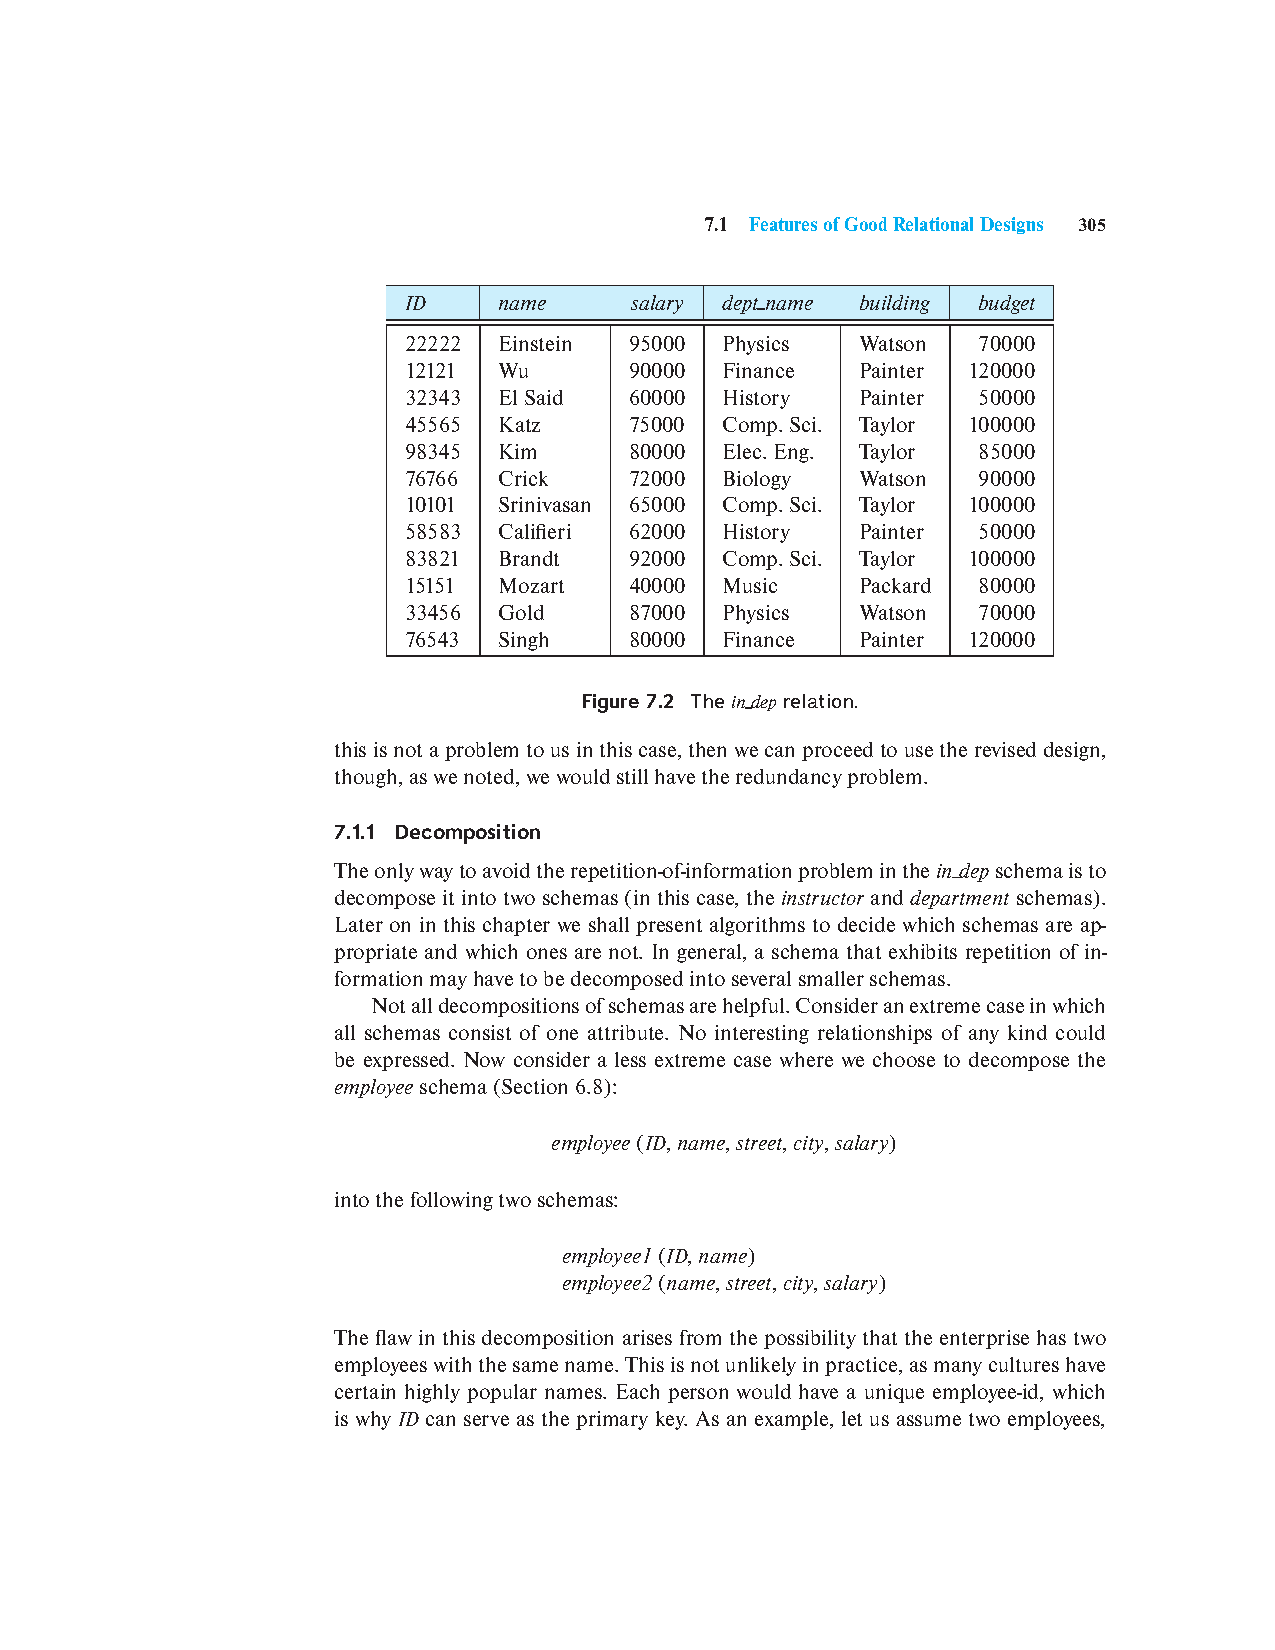
\includegraphics[width=.7\textwidth, trim={5cm 15.75cm 3.75cm 4.75cm}, clip]{figures/p305_in_dep}
            \end{center}
        \item There is repetition of information
        \item Need to use \texttt{\textbf{null}} values (if we add a new department with no instructors)
    \end{itemize}
\end{frame}

\begin{frame}{Decomposition}
    \begin{itemize}
        \item The only way to avoid the repetition-of-information problem in the \textit{in\_dep} schema is to decompose it into two schemas --\textit{instructor} and \textit{department} schemas.
        \item Not all decompositions are good. Suppose we decompose: \\
            \quad \texttt{employee(ID, name, street, city, salary)} \\
            into \\
            \quad \texttt{employee1 (ID, name)} \\
            \quad \texttt{employee2 (name, street, city, salary)} \\
            The problem arises when we have two employees with the same name.
        \item The next slide shows how we lose information --we cannot reconstruct the original employee relation-- and so, this is a \textbf{lossy decomposition}.
    \end{itemize}
\end{frame}

\begin{frame}{A Lossy Decomposition}
    \centering
    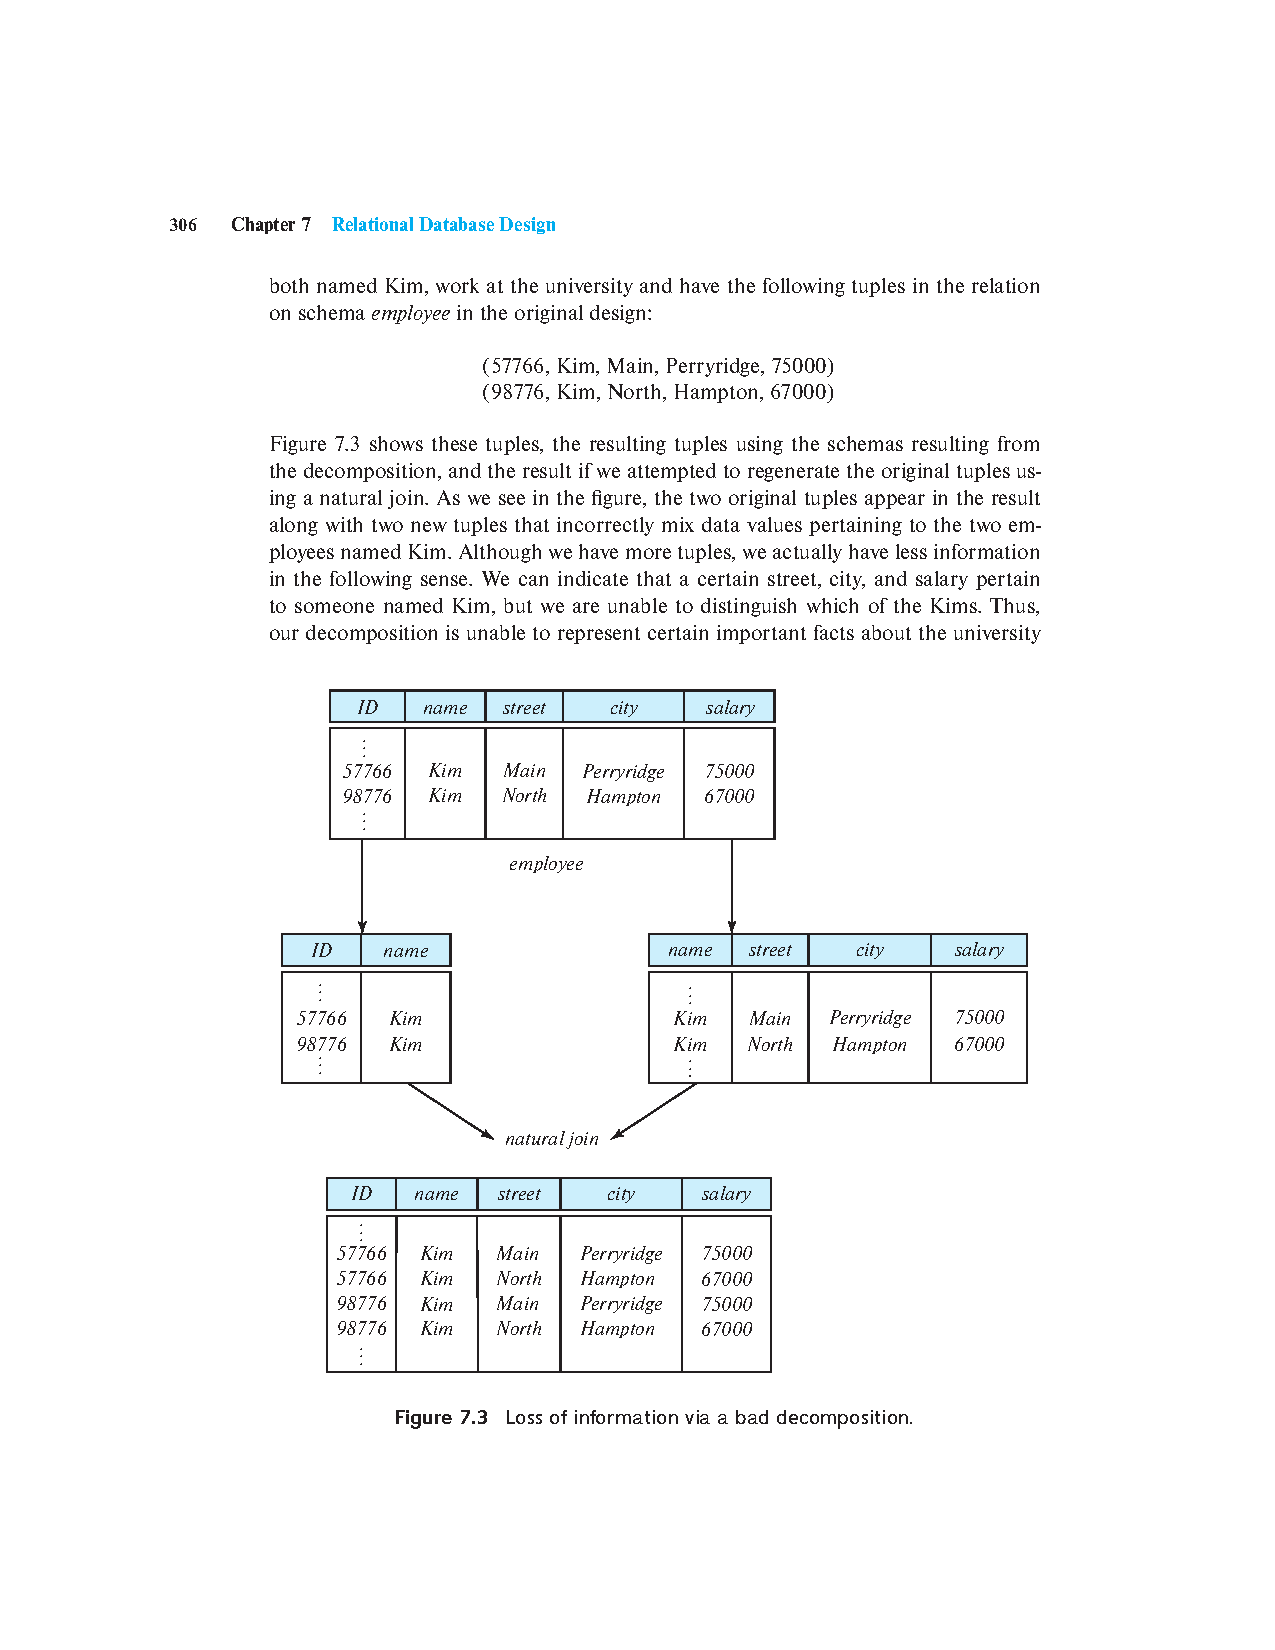
\includegraphics[width=0.85\textwidth, trim={3cm 2cm 4cm 11.25cm}, clip]{figures/p306_loss}
\end{frame}

\begin{frame}{Lossless Decomposition}
    \begin{itemize}
        \item Let $R$ be a relation schema and let $R_1$ and $R_2$ form a decomposition of $R$. That is $R = R_1 \bigcup R_2$.
        \item We say that the decomposition is a \textbf{lossless decomposition} if there is no loss of information by replacing $R$ with the two relation schemas $R_1 \bigcup R_2$.
        \item Formally,
            $$
                \Pi_{R_1}(r) \Join \Pi_{R_2}(r) = r
            $$
        \item And, conversely a decomposition is lossy if
            $$
                r \subset \Pi_{R_1}(r) \Join \Pi_{R_2}(r)
            $$
    \end{itemize}
\end{frame}

\begin{frame}{Example of Lossless Decomposition}
    \begin{itemize}
        \item Decomposition of $R = (A, B, C)$:
            $$
                R_1 = (A, B); R_2 = (B, C)
            $$
    \end{itemize}
    \centering
    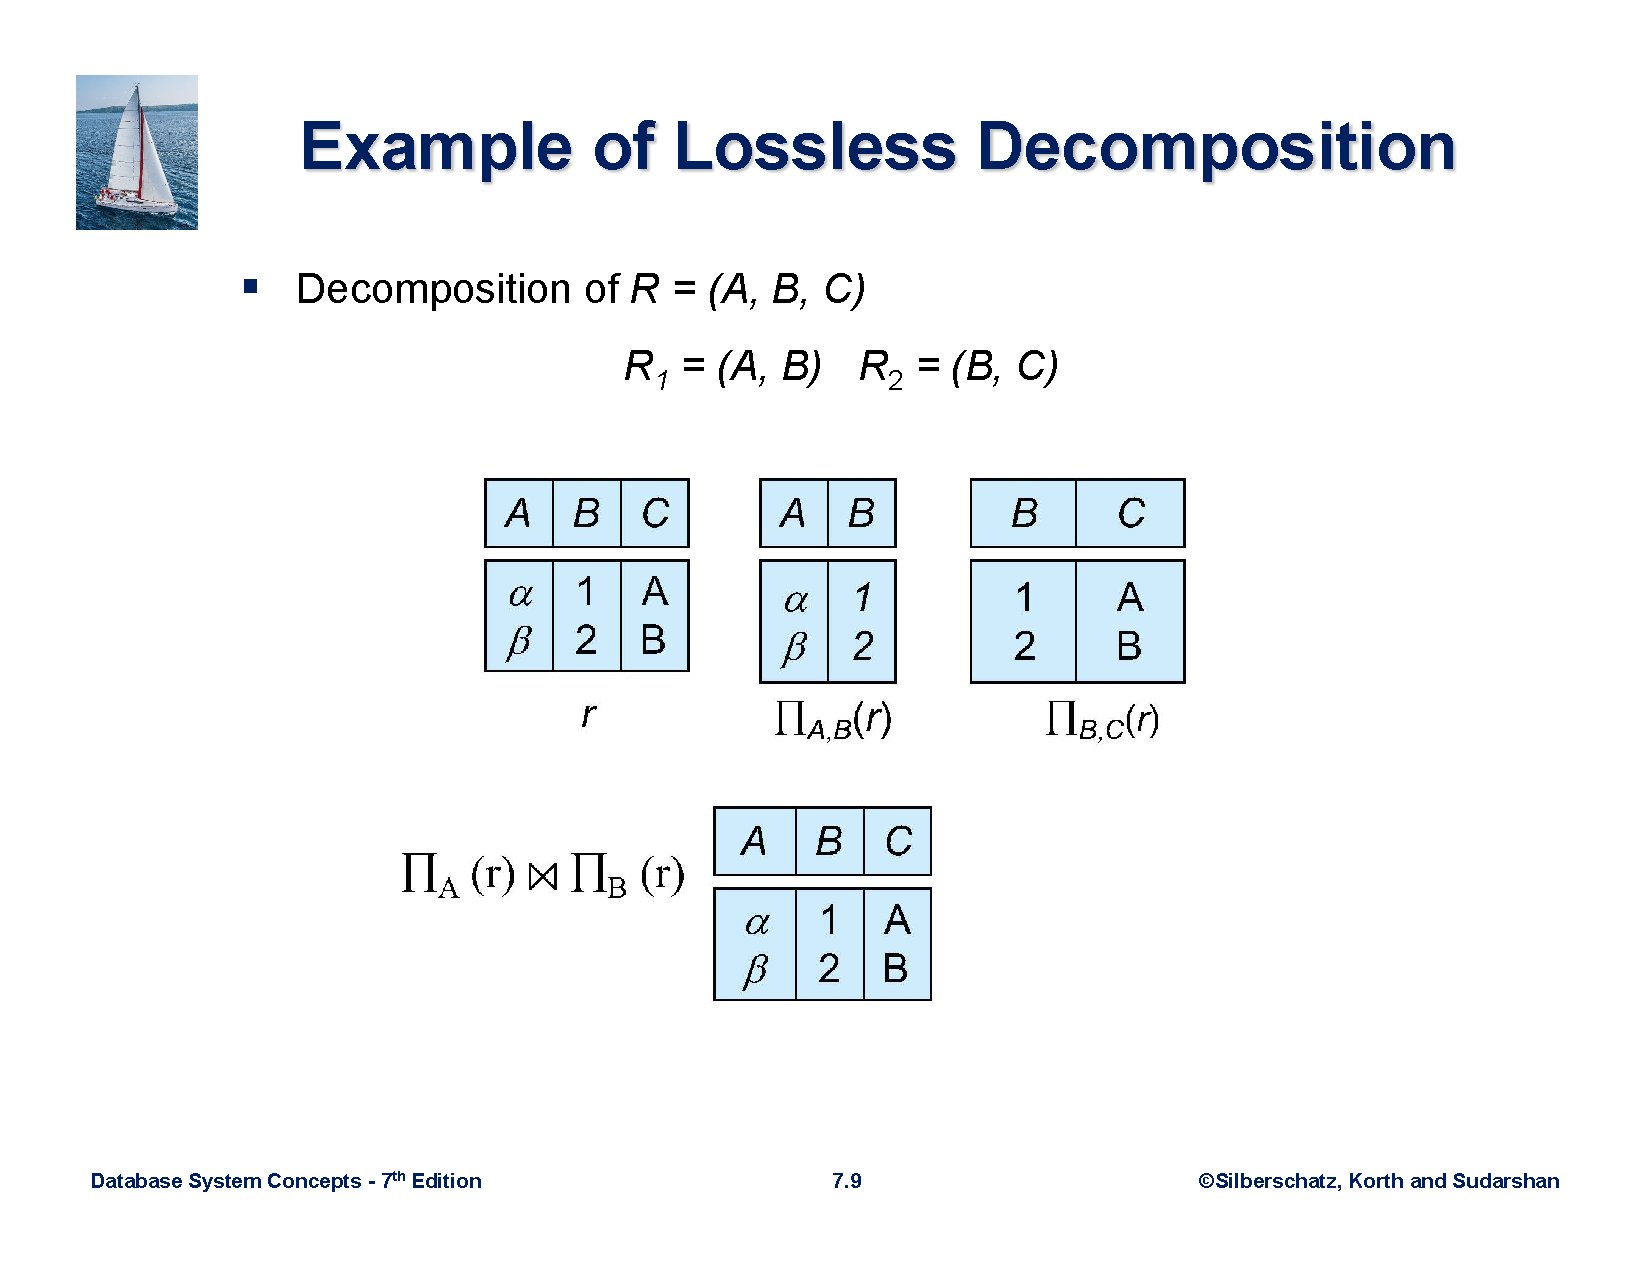
\includegraphics[width=\textwidth, trim={3cm 2cm 3cm 8cm}, clip]{figures/slide7_loss}
\end{frame}

\begin{frame}{Normalization Theory}
    \begin{itemize}
        \item Decide whether a particular relation $R$ is in ``good'' form.
        \item In the case that a relation $R$ is not in ``good'' form, decompose it into set of relations $\{R_1, R_2, \cdots, R_n\}$ such that,
        \begin{itemize}
            \item Each relation is in good form.
            \item The decomposition is a lossless decomposition.
        \end{itemize}
        \item Our theory is based on:
        \begin{enumerate}
            \item functional dependencies.
            \item multivalued dependencies.
        \end{enumerate}
    \end{itemize}
\end{frame}

\section{Functional Dependencies}

\begin{frame}{Functional Dependencies}
    \begin{itemize}
        \item There are usually a variety of constraints (rules) on the data in the real world.
        \item For example, some of the constraints that are expected to hold in a university database are:
        \begin{itemize}
            \item Students and instructors are uniquely identified by their ID.
            \item Each student and instructor has only one name.
            \item Each instructor and student is (primarily) associated with only one department.
            \item Each department has only one value for its budget, and only one associated building.
        \end{itemize}
    \end{itemize}
\end{frame}

\begin{frame}{Functional Dependencies (Cont.)}
    \begin{itemize}
        \item An instance of a relation that satisfies all such real-world constraints is called a \textbf{legal instance} of the relation.
        \item A legal instance of a database is one where all the relation instances are legal instances.
        \item Require that the value for a certain set of attributes determines uniquely the value for another set of attributes.
        \item A functional dependency is a generalization of the notion of a key.
    \end{itemize}
\end{frame}

\begin{frame}{Functional Dependencies Definition}
    \begin{itemize}
        \footnotesize
        \item Let $R$ be a relation schema
            \begin{equation*}
                \begin{align*}
                    \alpha \subseteq R \text{ and } \beta \subseteq R
                \end{align*}
            \end{equation*}
        \item The \textbf{functional dependency}
            $$
                \alpha \rightarrow \beta
            $$
            \textbf{holds on} $R$ if and only if for any legal relations $r(R)$, whenever any two tuples $t_1$ and $t_2$ of $r$ agree on the attributes $\alpha$, they also agree on the attributes $\beta$. That is,
            $$
                t_1[\alpha] = t_2[\alpha] \Rightarrow t_1[\beta] = t_2 [\beta]
            $$
        \item Example: Consider $r(A,B)$ with the following instance of $r$: \\
            \centering
            \begin{tabular}{|c|c|}
                \hline
                \textbf{A} & \textbf{B} \\ \hline
                1 & 4 \\ \hline
                1 & 5 \\ \hline
                3 & 7 \\ \hline
            \end{tabular}
        \item On this instance, $B \rightarrow A$ hold; $A \rightarrow B$ does \textbf{NOT} hold,
    \end{itemize}
\end{frame}

\begin{frame}{Closure of a Set of Functional Dependencies}
    \begin{itemize}
        \item Given a set $F$ set of functional dependencies, there are certain other functional dependencies that are logically implied by $F$.
        \begin{itemize}
            \item If $A \rightarrow B$ and $B \rightarrow C$, then we can infer that $A \rightarrow C$.
        \end{itemize}
        \item The set of \textbf{all} functional dependencies logically implied by $F$ is the \textbf{closure} of $F$.
        \item We denote the closure of $F$ by $F^+$.
    \end{itemize}
\end{frame}

\section{Decomposition Using Functional Dependencies}

\begin{frame}{Keys and Functional Dependencies}
    \begin{itemize}
        \item $K$ is a superkey for relation schema $R$ if and only if $K \rightarrow R$.
        \item $K$ is a primary key for $R$ if and only if:
        \begin{itemize}
            \item $K \rightarrow R$, and
            \item for no $\alpha \subset K, \alpha \rightarrow R$
        \end{itemize}
        \item Functional dependencies allow us to express constraints that cannot be expressed using superkeys. Consider the schema:
            \begin{center}
                \texttt{\footnotesize in\_dep(ID, name, salary, dept\_name, building, budget)}.
            \end{center}
        We expect these functional dependencies to hold:
            \begin{equation*}
                \begin{align*}
                    dept\_name \rightarrow& building \\
                    ID \rightarrow& building
                \end{align*}
            \end{equation*}
        but would not expect the following to hold:
            \begin{equation*}
                \begin{align*}
                    dept\_name \rightarrow& salary
                \end{align*}
            \end{equation*}
    \end{itemize}
\end{frame}

\begin{frame}{Use of Functional Dependencies}
    \begin{itemize}
        \item We use functional dependencies to:
        \begin{itemize}
            \item To test relations to see if they are legal under a given set of functional dependencies.
            \begin{itemize}
                \item If a relation $r$ is legal under a set $F$ of functional dependencies, we say that $r$ \textbf{satisfies} $F$.
            \end{itemize}
            \item To specify constraints on the set of legal relations.
            \begin{itemize}
                \item We say that $F$ \textbf{holds on} $R$ if all legal relations on $R$ satisfy the set of functional dependencies $F$.
            \end{itemize}
        \end{itemize}
        \item Note: A specific instance of a relation schema may satisfy a functional dependency even if the functional dependency does not hold on all legal instances.
        \begin{itemize}
            \item For example, a specific instance of \textit{instructor} may, by chance, satisfy
            $$
                name \rightarrow ID.
            $$
        \end{itemize}
    \end{itemize}
\end{frame}

\begin{frame}{Trivial Functional Dependencies}
    \begin{itemize}
        \item A functional dependency is \textbf{trivial} if it is satisfied by all instances of a relation.
        \begin{itemize}
            \item Example:
            \begin{itemize}
                \item $ID, name \rightarrow ID$
                \item $name \rightarrow name$
            \end{itemize}
            \item In general, $\alpha \rightarrow \beta$ is trivial if $\beta \subseteq \alpha$.
        \end{itemize}
    \end{itemize}
\end{frame}

\begin{frame}{Lossless Decomposition}
    \begin{itemize}
        \item We can use functional dependencies to show when certain decomposition are lossless.
        \item For the case of $R = (R_1, R_2)$, we require that for all possible relations $r$ on schema $R$
            $$
                r = \Pi_{R_1}(r) \Join \Pi_{R_2}(r)
            $$
        \item A decomposition of $R$ into $R_1$ and $R_2$ is lossless decomposition if at least one of the following dependencies is in $F^+$:
        \begin{equation*}
            \begin{align*}
                R_1 \bigcap R_2 \rightarrow& R_1 \\
                R_1 \bigcap R_2 \rightarrow& R_2
            \end{align*}
        \end{equation*}
        \item The above functional dependencies are a sufficient condition for lossless join decomposition; the dependencies are a necessary condition only if all constraints are functional dependencies.
    \end{itemize}
\end{frame}

\begin{frame}{Example\footnote{Note: $B \rightarrow BC$ is a shorthand notation for $B \rightarrow \{B, C\}$.}}
    \begin{itemize}
        \item $R = (A, B, C)$
            \begin{equation*}
                \begin{align*}
                    F = \{  A \rightarrow& B \\
                            B \rightarrow& C\}
                \end{align*}
            \end{equation*}

        \item $R_1 = (A, B)$; $R_2 = (B, C)$ \\
            \text{Lossless decomposition:} \\
            $R_1 \bigcap R_2 = \{B\}$  and $B \rightarrow BC$ holds.
        \item $R_1 = (A, B)$; $R_2 = (A, C)$ \\
            \text{Lossless decomposition:} \\
            $R_1 \bigcap R_2 = \{A\}$  and $A \rightarrow AC$ holds.
    \end{itemize}
\end{frame}

\begin{frame}{Dependency Preservation}
    \begin{itemize}
        \item Testing functional dependency constraints each time the database is updated can be costly,
        \item It is useful to design the database in a way that constraints can be tested efficiently.
        \item If testing a functional dependency can be done by considering just one relation, then the cost of testing this constraint is low.
        \item When decomposing a relation it is possible that it is no longer possible to do the testing without having to perform a Cartesian Produced.
        \item A decomposition that makes it computationally hard to enforce functional dependency is said to be NOT \textbf{dependency preserving}.
    \end{itemize}
\end{frame}

\begin{frame}{Dependency Preservation Example}
    \begin{itemize}
        \item Consider a schema:
            \begin{center}
                \texttt{dept\_advisor(s\_ID, i\_ID, department\_name)}
            \end{center}
        \item With function dependencies:
            \begin{center}
                $i\_ID \rightarrow dept\_name$ \\
                $s\_ID, dept\_name \rightarrow i\_ID$
            \end{center}
        \item In the above design we are forced to repeat the department name once for each time an instructor participates in a \textit{dept\_advisor} relationship.
        \item To fix this, we need to decompose \textit{dept\_advisor}.
        \item Any decomposition will not include all the attributes in:
            \begin{center}
                $s\_ID, dept\_name \rightarrow i\_ID$
            \end{center}
        \item Thus, the composition NOT be dependency preserving.
    \end{itemize}
\end{frame}

\section{Normal Forms}

\begin{frame}{Boyce-Codd Normal Form}
    \begin{itemize}
        \item A relation schema $R$ is in BCNF with respect to a set $F$ of functional dependencies if for all functional dependencies in $F^+$ of the form:
        $$
            \alpha \rightarrow \beta
        $$
        where $\alpha \subseteq R$ and $\beta \subseteq R$, at least one of the following holds:
        \begin{itemize}
            \item $\alpha \rightarrow \beta$ is trivial (i.e., $\beta \subseteq \alpha$)
            \item $\alpha$ is a superkey for $R$.
        \end{itemize}
    \end{itemize}
\end{frame}

\begin{frame}{Boyce-Codd Normal Form (Cont.)}
    \begin{itemize}
        \item Example schema that is not in BCNF: \\
            \begin{center}
                \texttt{\footnotesize in\_dep (ID, name, salary, dept\_name, building, budget)}
            \end{center}
        because :
        \begin{itemize}
            \item $dept\_name \rightarrow building, budget$
            \begin{itemize}
                \item holds on \texttt{in\_dep}
                \item but...
            \end{itemize}
            \item \textit{dept\_name} is not a superkey.
        \end{itemize}
        \item When decompose \texttt{in\_dept} into \texttt{instructor} and \texttt{department}:
        \begin{itemize}
            \item \texttt{instructor} is in BCNF.
            \item \texttt{department} is in BCNF.
        \end{itemize}
    \end{itemize}
\end{frame}

\begin{frame}{Decomposing a Schema into BCNF}
    \begin{itemize}
        \item Let $R$ be a schema that is not in BCNF. Let $\alpha \rightarrow \beta$ be the Fuctional Dependency that causes a violation of BCNF.
        \item We decompose $R$ into:
            \begin{itemize}
                \item $(\alpha \bigcup \beta)$
                \item $(R - (\beta - \alpha))$
            \end{itemize}
        \item In our example of \texttt{in\_dep},
            \begin{itemize}
                \item $\alpha = dept\_name$
                \item $\beta = building, budget$
            \end{itemize}
        and \texttt{in\_dep} is replaced by
            \begin{itemize}
                \item $(\alpha \bigcup \beta) = (dept\_name, building, budget)$
                \item $(R - (\beta - \alpha)) = (ID, name, salary, dept\_name)$
            \end{itemize}
    \end{itemize}
\end{frame}

\begin{frame}{BCNF and Dependency Preservation}
    \begin{itemize}
        \item It is not always possible to achieve both BCNF and dependency preservation.
        \item Consider a schema:
            \begin{center}
                \texttt{dept\_advisor(s\_ID, i\_ID, department\_name)}
            \end{center}
        \item With function dependencies:\\
            \begin{tabular}{r l}
                $i\_ID \rightarrow$ & $dept\_name$ \\
                $s\_ID, dept\_name \rightarrow$ & $i\_ID$
            \end{tabular}
        \item \texttt{dept\_advisor} is not in BCNF:
            \begin{itemize}
                \item \textit{i\_ID} is not a superkey.
            \end{itemize}
        \item Any decomposition of \texttt{dept\_advisor} will not include all the attributes in: \\
            \begin{tabular}{r l}
                $s\_ID, dept\_name \rightarrow$ & $i\_ID$
            \end{tabular}
        \item Thus, the composition is NOT be dependency preserving.
    \end{itemize}
\end{frame}

\begin{frame}{Third Normal Form}
    \begin{itemize}
        \item A relation schema R is in \textbf{third normal form (3NF)} if for all:
            \begin{center}
                $\alpha \rightarrow \beta$ in $F^+$
            \end{center}
        at least one of the following holds:
            \begin{itemize}
                \item $\alpha \rightarrow \beta$ is trivial (i.e., $\beta \in \alpha$).
                \item $\alpha$ is a superkey for $R$.
                \item Each attribute $A$ in $\beta - \alpha$ is contained in a candidate key\footnote{NOTE: each attribute may be in a different candidate key.} for $R$.
            \end{itemize}
        \item If a relation is in BCNF it is in 3NF (since in BCNF one of the first two conditions above must hold).
        \item Third condition is a minimal relaxation of BCNF to ensure dependency preservation (will see why later).
    \end{itemize}
\end{frame}

\begin{frame}{3NF Example}
    \begin{itemize}
        \item Consider a schema:
            \begin{center}
                \texttt{dept\_advisor(s\_ID, i\_ID, dept\_name)}
            \end{center}
        \item With function dependencies:
            \begin{equation*}
                \begin{align*}
                    i\_ID \rightarrow& dept\_name \\
                    s\_ID, dept\_name \rightarrow& i\_ID
                \end{align*}
            \end{equation*}
        \item Two candidate keys = $\{s\_ID, dept\_name\}$, $\{s\_ID, i\_ID\}$
        \item We have seen before that \texttt{dept\_advisor} is not in BCNF.
        \item R, however, is in 3NF:
            \begin{itemize}
                \item $s\_ID$, $dept\_name$ is a superkey,
                \item $i\_ID \rightarrow dept\_name$ and $i\_ID$ is NOT a superkey, but:
                    \begin{itemize}
                        \item ${dept\_name} - {i\_ID} = {dept\_name}$ and
                        \item $dept\_name$ is contained in a candidate key.
                    \end{itemize}
            \end{itemize}
    \end{itemize}
\end{frame}

\begin{frame}{Redundancy in 3NF}
    \begin{itemize}
        \item Consider the schema $R$ below, which is in 3NF:
            \begin{itemize}
                \item $R = (J, K, L )$,
                \item $F = \{JK \rightarrow L, L \rightarrow K \}$,
                \item And an instance table:
                    \begin{center}
                        \begin{tabular}{| c | c | c |}
                            \hline
                            J     & L     & K     \\
                            \hline
                            $j_1$ & $l_1$ & $k_1$ \\
                            $j_2$ & $l_1$ & $k_1$ \\
                            $j_3$ & $l_1$ & $k_1$ \\
                            \texttt{\textbf{null}} & $l_2$ & $k_2$ \\
                            \hline
                        \end{tabular}
                    \end{center}
            \end{itemize}
        \item What is wrong with the table? \pause
            \begin{itemize}
                \item Repetition of information,
                \item Need to use \texttt{\textbf{null}} values (e.g., to represent the relationship $l_2$, $k_2$ where there is no corresponding value for $J$)
            \end{itemize}
    \end{itemize}
\end{frame}

\begin{frame}{Comparison of BCNF and 3NF}
    \begin{itemize}
        \item Advantages to 3NF over BCNF. It is always possible to obtain a 3NF design without sacrificing losslessness or dependency preservation.
        \item Disadvantages to 3NF.
            \begin{itemize}
                \item We may have to use \texttt{\textbf{null}} values to represent some of the possible meaningful relationships among data items.
                \item There is the problem of repetition of information.
            \end{itemize}
    \end{itemize}
\end{frame}

\begin{frame}{Goals of Normalization}
    \begin{itemize}
        \item Let $R$ be a relation scheme with a set $F$ of functional dependencies.
        \item Decide whether a relation scheme $R$ is in ``good'' form.
        \item In the case that a relation scheme $R$ is not in ``good'' form, decompose it into a set of relation scheme $\{R_1, R_2, \cdots, R_n\}$ such that:
            \begin{itemize}
                \item Each relation scheme is in good form,
                \item The decomposition is a lossless decomposition,
                \item Preferably, the decomposition should be dependency preserving.
            \end{itemize}
    \end{itemize}
\end{frame}

\begin{frame}{How good is BCNF?}
    \begin{itemize}
        \item There are database schemas in BCNF that do not seem to be sufficiently normalized...
        \item Consider a relation:
            \begin{center}
                \texttt{inst\_info(ID, child\_name, phone)}
            \end{center}
        where an instructor may have more than one phone and can have multiple children.
        \item Instance of \texttt{inst\_info}
            \begin{center}
                \begin{tabular}{ c c c}
                    \hline
                    \textbf{ID} & \textbf{child\_name} & \textbf{phone} \\
                    \hline
                    99999 & David   & 512-555-1234 \\
                    99999 & David   & 512-555-4321 \\
                    99999 & William & 512-555-1234 \\
                    99999 & William & 512-555-4321 \\
                    \hline
                \end{tabular}
            \end{center}
    \end{itemize}
\end{frame}

\begin{frame}{How good is BCNF? (Cont.)}
    \begin{itemize}
        \item There are no non-trivial functional dependencies and therefore the relation is in BCNF.
        \item Insertion anomalies -- i.e., if we add a phone 981-992-3443 to 99999, we need to add two tuples:
            \begin{center}
                \begin{tabular}{l}
                    (99999, David, 981-992-3443) \\
                    (99999, William, 981-992-3443)
                \end{tabular}
            \end{center}
    \end{itemize}
\end{frame}

\begin{frame}{Higher Normal Forms}
    \begin{itemize}
        \item It is better to decompose \texttt{inst\_info} into:
            \begin{itemize}
                \item \texttt{inst\_child}
                    \begin{center}
                        \begin{tabular}{r r}
                            \hline
                            \textbf{ID} & \textbf{child\_name} \\
                            \hline
                            99999 & David   \\
                            99999 & William \\
                            \hline
                        \end{tabular}
                    \end{center}
                \item \texttt{inst\_phone}
                    \begin{center}
                        \begin{tabular}{r r}
                            \hline
                            \textbf{ID} & \textbf{phone} \\
                            \hline
                            99999 & 512-555-1234 \\
                            99999 & 512-555-4321 \\
                            \hline
                        \end{tabular}
                    \end{center}
            \end{itemize}
        \item This suggests the need for higher normal forms, such as Fourth Normal Form (4NF), which we shall see later
    \end{itemize}
\end{frame}

\section{Functional Dependency Theory}

\begin{frame}{Functional-Dependency Theory Roadmap}
    \begin{itemize}
        \item We now consider the formal theory that tells us which functional dependencies are implied logically by a given set of functional dependencies.
        \item We then develop algorithms to generate lossless decompositions into BCNF and 3NF.
        \item We then develop algorithms to test if a decomposition is dependency-preserving.
    \end{itemize}
\end{frame}

\begin{frame}{Closure of a Set of Functional Dependencies}
    \begin{itemize}
        \item Given a set F set of functional dependencies, there are certain other functional dependencies that are logically implied by F.
            \begin{itemize}
                \item If $A \rightarrow B$ and $B \rightarrow C$, then we can infer that $A \rightarrow C$
                \item etc.
            \end{itemize}
        \item The set of all functional dependencies logically implied by $F$ is the closure of $F$.
        \item We denote the closure of $F$ by $F^+$.
    \end{itemize}
\end{frame}

\begin{frame}{Closure of a Set of Functional Dependencies}
    \begin{itemize}
        \item We can compute $F^+$, the closure of $F$, by repeatedly applying \textbf{Armstrong's Axioms}:
            \begin{itemize}
                \item \textbf{Reflexive rule}: if $\beta \subseteq \alpha$, then $\alpha \rightarrow \beta$,
                \item \textbf{Augmentation rule}: if $\alpha \rightarrow \beta$, then $\gamma \alpha \rightarrow \gamma \beta$,
                \item \textbf{Transitivity rule}: if $\alpha \rightarrow \beta$, and $\beta \rightarrow \gamma$, then $\alpha \rightarrow \gamma$.
            \end{itemize}
        \item These rules are:
            \begin{itemize}
                \item \textbf{sound} -- generate only functional dependencies that actually hold, and
                \item \textbf{complete} -- generate all functional dependencies that hold.
            \end{itemize}
    \end{itemize}
\end{frame}

\begin{frame}{Example of $F^+$}
    \begin{itemize}
        \item $R = (A, B, C, G, H, I)$
            \begin{equation*}
                \begin{align*}
                    F=\{A \rightarrow& B \\
                        A \rightarrow& C \\
                       CG \rightarrow& H \\
                       CG \rightarrow& I \\
                        B \rightarrow& H\} \\
                \end{align*}
            \end{equation*}
        \item Some members of $F^+$
            \begin{itemize}
                \item $A \rightarrow H$ by transitivity from $A \rightarrow B$ and $B \rightarrow H$.
                \item $AG \rightarrow I$ by augmenting $A \rightarrow C$ with $G$, to get $AG \rightarrow CG$ and then transitivity with $CG \rightarrow I$.
                \item $CG \rightarrow HI$ by augmenting $CG \rightarrow I$ to infer $CG \rightarrow CGI$, and augmenting of $CG \rightarrow H$ to infer $CGI \rightarrow HI$, and then transitivity.
            \end{itemize}
    \end{itemize}
\end{frame}

\begin{frame}{Closure of a Set of Functional Dependencies (Cont.)}
    \begin{itemize}
        \item Additional rules:
            \begin{itemize}
                \item \textbf{Union rule}: If $\alpha \rightarrow \beta$ holds and $\alpha \rightarrow \gamma$ holds, then $\alpha \rightarrow \beta \gamma$ holds.
                \item \textbf{Decomposition rule}: If $\alpha \rightarrow \beta \gamma$ holds, then $\alpha \rightarrow \beta$ holds and $\alpha \rightarrow \gamma$ holds.
                \item \textbf{Pseudotransitivity rule}: If $\alpha \rightarrow \beta$ holds and $\gamma \beta \rightarrow \delta$ holds, then $\alpha \gamma \rightarrow \delta$ holds.
            \end{itemize}
        \item The above rules can be inferred from Armstrong's axioms.
    \end{itemize}
\end{frame}

\begin{frame}{Procedure for Computing $F^+$}
    \begin{itemize}
        \item To compute\footnote{NOTE: We shall see an alternative procedure for this task later.} the closure of a set of functional dependencies $F$:
    \end{itemize}
    \centering
    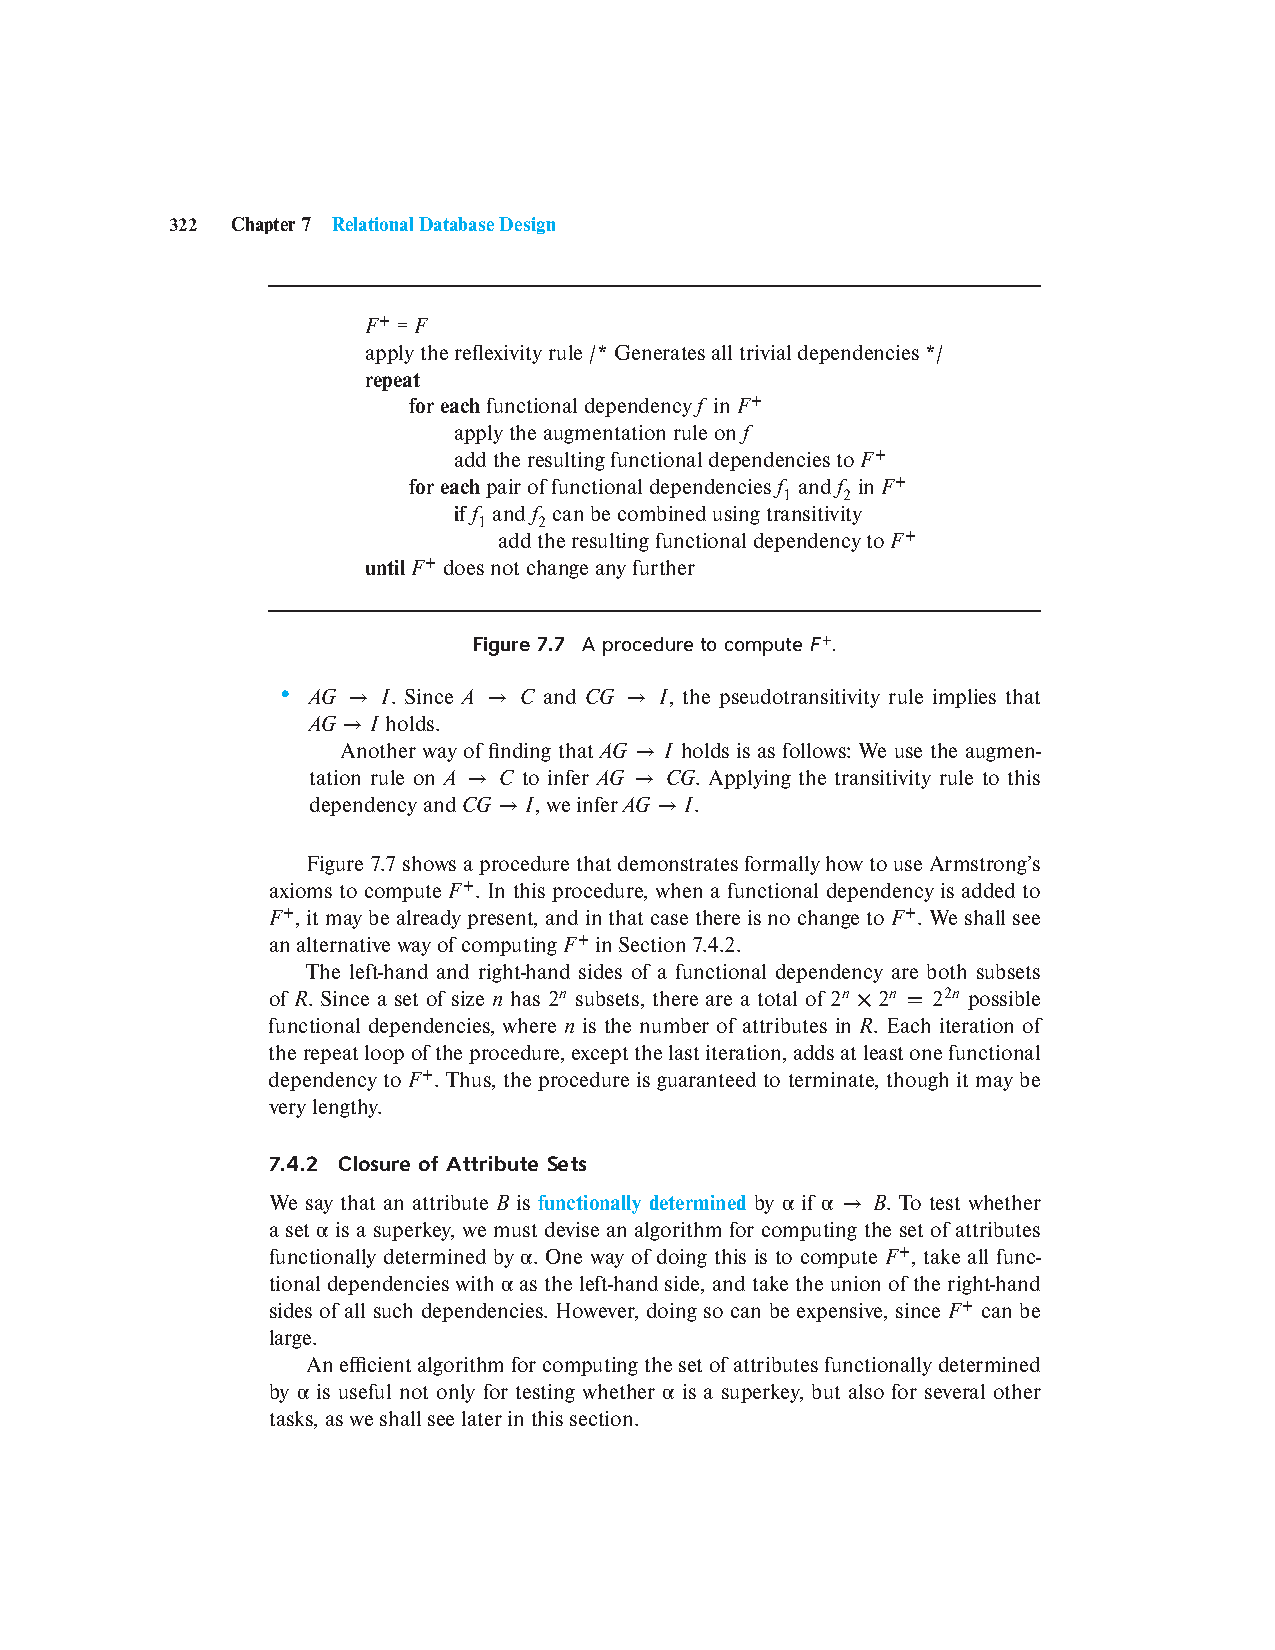
\includegraphics[width=\textwidth, trim={4cm 16.5cm 4cm 4.5cm}, clip]{figures/p322_Fplus_procedure}
\end{frame}

\begin{frame}{Closure of Attribute Sets}
    \begin{itemize}
        \item Given a set of attributes $\alpha$, define the closure of $\alpha$ under $F$ (denoted by $\alpha^+$) as the set of attributes that are functionally determined by $\alpha$ under $F$.
        \item Algorithm to compute $\alpha^+$, the closure of $\alpha$ under $F$:
    \end{itemize}
    \centering
    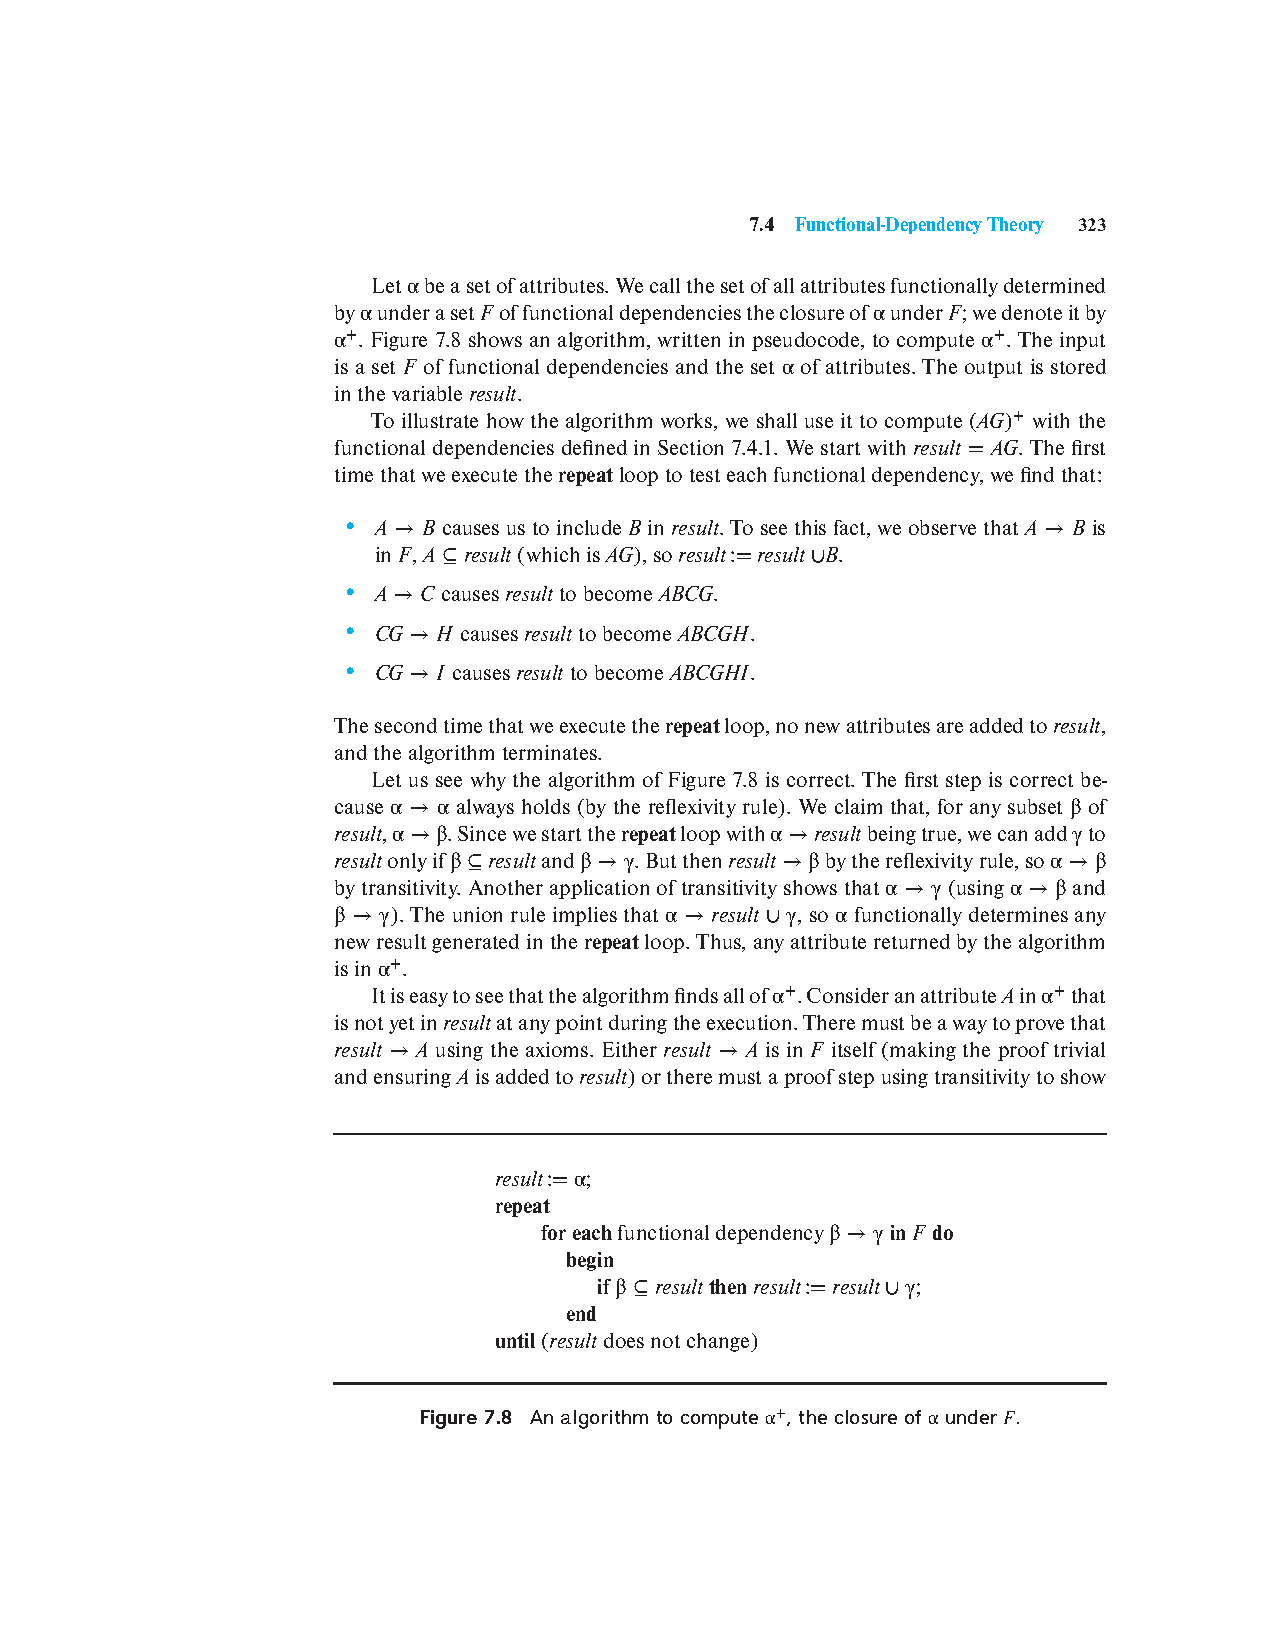
\includegraphics[width=0.9\textwidth, trim={6.5cm .75cm 3.5cm 19cm}, clip]{figures/p323_Aplus_procedure}
\end{frame}

\begin{frame}{Example of Attribute Set Closure}
    \footnotesize
    \begin{itemize}
        \item $R = (A, B, C, G, H, I)$
            \begin{equation*}
                \begin{align*}
                    F = \{  A   \rightarrow& B \\
                            A   \rightarrow& C \\
                            CG  \rightarrow& H \\
                            CG  \rightarrow& I \\
                            B   \rightarrow& H\} \\
                \end{align*}
            \end{equation*}
        \item $(AG)^+$
            \begin{enumerate}
                \item result = $AG$.
                \item result = $ABCG(A \rightarrow C$ and $A \rightarrow B)$.
                \item result = $ABCGH(CG \rightarrow H$ and $CG \subseteq AGBC)$.
                \item result = $ABCGHI(CG \rightarrow I$ and $CG \subseteq AGBCH)$.
            \end{enumerate}
        \item Is $AG$ a candidate key?
            \begin{enumerate}
                \item Is $AG$ a super key?
                    \begin{enumerate}
                        \item Does $AG \rightarrow R$? $==$ Is $R \supseteq (AG)^+$.
                    \end{enumerate}
                \item Is any subset of $AG$ a superkey?
                    \begin{enumerate}
                        \item Does $A \rightarrow R$? $==$ Is $R \supseteq (A)^+$.
                        \item Does $G \rightarrow R$? $==$ Is $R \supseteq (G)^+$.
                        \item In general: check for each subset of size $n-1$.
                    \end{enumerate}
            \end{enumerate}
    \end{itemize}
\end{frame}



























\begin{frame}{}
\end{frame}

\section{Algorithms for Decomposition using Functional Dependencies}
\section{Decomposition Using Multivalued Dependencies}
\section{More Normal Form}
\section{Atomic Domains and First Normal Form}
\section{Database-Design Process}
\section{Modeling Temporal Data}

% \begin{frame}[fragile]{}
%     \begin{minted}
%     [tabsize=4, obeytabs, frame=lines, framesep=2mm, baselinestretch=1.2, bgcolor=LightGray, fontsize=\scriptsize]{sql}
%     \end{minted}
% \end{frame}

\begin{frame}{}
     \centering
     \Huge End of Chapter 7.
\end{frame}

\section*{Takeaways}

% Tim Duncan's Top 5 Fundamental Takeaways of the Today's Class
\begin{frame}{TDT5FTOTTC}
    \centering
    
\includegraphics[width=0.75\textwidth]{figures/tim.png}
\end{frame}

\begin{frame}{Top 5 Fundamental Takeaways}
    \small
    \begin{enumerate} \pause
        \item[5]
    \end{enumerate}
\end{frame}

\begin{frame}{Database System Concepts}
    \centering
    
\includegraphics[width=0.5\textwidth]{figures/book_cover.jpg} \\
    \vspace{5mm}
    {
        \tiny
        Content has been extracted from \textit{Database System Concepts}, Seventh Edition, by Silberschatz, Korth and Sudarshan. Mc Graw Hill Education. 2019.\\
        Visit \url{https://db-book.com/}.\\
    }
\end{frame}

\end{document}
